\subsection{Smart Grapple State Estimation}
The goal of state estimation is to compute the approximate position and velocity of the \gls{usg}. This information is required for trajectory tracking during locomotion of the robot, as described in Section~\ref{sec:trackingState}. The proposed approach leverages an \gls{ekf} on the measured sensor data to achieve state estimation.

\textbf{Sensor fusion.}
Two types of sensors are used as data sources for state estimation: an \gls{imu} and a \gls{dvl}. The \gls{imu} provides measurements of linear acceleration and angular velocity, while the \gls{dvl} provides measurements of linear and angular velocity and altitude of the vehicle relative to the seabed. In order to increase the precision of state estimation, the \gls{imu} and \gls{dvl} measurements are fused together via the \gls{ekf} \cite{10.5555/897831}.

\begin{figure}[ht]
	\centering
	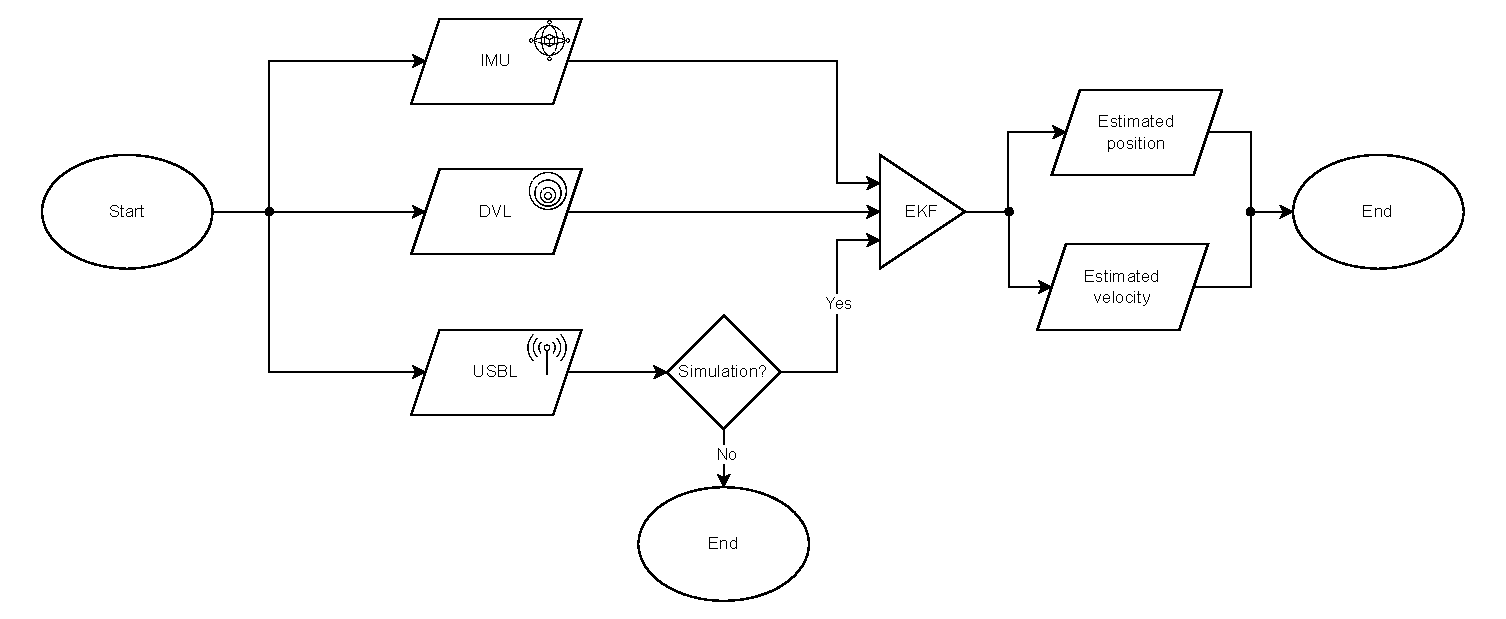
\includegraphics[width=\textwidth]{img/state_estimation_flowchart.drawio.pdf}
	\caption{Information flow of the state estimation}
	\label{fig:stateEstimationFlowchart}
\end{figure}

\textbf{Implementation.}
The \textit{robot\_localization} package, developed by Charles River Analytics, is used to implement the \gls{ekf} \cite{MooreStouchKeneralizedEkf2014}. It is an open-source package that provides a basic framework for localization tasks that can be easily adapted to different robotic systems such as the \gls{usg}. The main benefits of this package are:
\begin{itemize}
    \item Supports ROS 2 out-of-the-box,
    \item Handles an unlimited number of inputs from multiple sensor types,
    \item Allows 3D localization,
    \item Provides higher control over the sensor data and how it impacts the estimation.
\end{itemize}

\textbf{Simulation.}
The state estimation module is part of the digital twin. The data sources for sensor fusion in simulation are slightly different as they also include \gls{gnss} measurements. These measurements are used to emulate a \gls{usbl} acoustic positioning system, which will be added to the \gls{usg} hardware in the future. For more details on the digital twin, refer to Section~\ref{sec:sim}.